\ChapterImageStar[cap:caracterizacionGRID]{Caracterización del GRID}{./images/fondo.png}\label{cap:caracterizacionGRID}
\mbox{}\\
\noindent
El Grupo de Investigación en Redes, Información y Distribución (GRID) de la Universidad del Quindío se alinea con los objetivos misionales de la institución en los ámbitos de educación, investigación y extensión. Entre sus principales intereses se destaca la oferta de servicios tecnológicos avanzados para la comunidad académica, con especial atención a los estudiantes del programa de Ingeniería de Sistemas y Computación, quienes encuentran en el grupo un espacio de formación, experimentación e innovación en temas relacionados con infraestructura, ingeniería de software y tecnologías emergentes.
La caracterización del GRID es fundamental para comprender su estructura organizacional, sus capacidades técnicas y sus necesidades específicas frente a al desarrollo e implementación de una notacion de diseño de infraestructura de \TI. En este sentido, a continuación se presenta un análisis de los principales aspectos que definen el contexto institucional y tecnológico del grupo.

\section{Análisis de stakeholders del GRID}
\noindent
Con el propósito de identificar los actores internos y externos que inciden en el desarrollo de las actividades del grupo, se llevó a cabo un análisis de stakeholders. Este proceso permitió reconocer los distintos intereses, roles y niveles de influencia que cada actor ejerce en relación con la aplicación de notaciones de diseño de infraestructura de \TI. Entre los principales stakeholders identificados se encuentran los investigadores del grupo, los estudiantes de pregrado y posgrado, los docentes de la Facultad de Ingeniería y, en un ámbito más amplio, la comunidad académica de la Universidad del Quindío.
\\
\noindent
La tabla \ref{tab:stakeholders} presenta el análisis de los principales interesados en el desarrollo e implementación de una notación para el modelado de infraestructura de TI en el contexto del programa de Ingeniería de Sistemas y Computación de la Universidad del Quindío. En ella se identifican los actores internos y externos que intervienen en el proyecto, detallando su rol, tipo de relación, nivel de impacto, poder de influencia, interés y grado de compromiso con la iniciativa.

El análisis evidencia una estructura de actores diversa, donde el Grupo de Investigación GRID se consolida como el principal interesado y beneficiario. Su alta influencia, interés y compromiso reflejan su papel protagónico en la definición, validación y adopción de los modelos de infraestructura propuestos, además de su responsabilidad en garantizar la coherencia técnica y metodológica del proyecto. Su involucramiento resulta esencial para alinear los resultados con los objetivos estratégicos del grupo y con las necesidades reales de gestión tecnológica y arquitectónica.

En un segundo nivel de relevancia se ubican los docentes e investigadores de la Facultad de Ingeniería, quienes actúan como usuarios clave del lenguaje y promotores de su aplicación en el ámbito académico. Aunque su poder de decisión es moderado, su participación es determinante para consolidar la utilidad práctica del modelo y facilitar su incorporación en actividades de formación, proyectos de aula e investigación aplicada. Este grupo demanda especial atención en términos de documentación, capacitación y herramientas que simplifiquen la comprensión y el uso de las notaciones.

Por su parte, los estudiantes se configuran como beneficiarios directos del proyecto, dado que la notación propuesta fortalecerá sus competencias en arquitectura empresarial, infraestructura de TI y diseño conceptual. Su impacto individual es bajo, pero su participación en la validación práctica de los modelos será clave para medir la usabilidad y la adopción dentro del entorno educativo.

El Programa de Ingeniería de Sistemas y Computación cumple un rol estratégico como facilitador institucional, con alta capacidad de influencia en la integración del proyecto dentro de la estructura académica de la Universidad. Su respaldo será determinante para garantizar la sostenibilidad y expansión del uso de la notación en otros espacios curriculares o de investigación.

Finalmente, la comunidad académica y profesional de arquitectura empresarial, junto con los grupos de investigación aliados, representan un público externo de interés. Aunque su poder de decisión es limitado, aportan conocimiento metodológico, estándares y buenas prácticas que enriquecen el desarrollo del modelo. Su interacción con el proyecto podría generar sinergias valiosas y contribuir a la validación de la notación en escenarios más amplios, fortaleciendo así la proyección institucional y científica de la propuesta.

\begin{table}[H]
	\centering
	\fontsize{7}{7}\selectfont
	\setlength{\tabcolsep}{3pt}
	\renewcommand{\arraystretch}{1.4}
	\begin{tabularx}{\textwidth}{%
		>{\raggedright\arraybackslash}p{1.7cm}  
		>{\raggedright\arraybackslash}p{1.5cm}    
		>{\raggedright\arraybackslash}p{2.3cm}  
		>{\raggedright\arraybackslash}p{1.4cm}  
		>{\raggedright\arraybackslash}p{2.0cm}  
		>{\raggedright\arraybackslash}p{2.5cm}    
		>{\raggedright\arraybackslash}p{2.0cm}} 
		\toprule
		\textbf{Interesado} & \textbf{Rol} & \textbf{Relación} & \textbf{Impacto} & \textbf{Poder de influencia} & \textbf{Interés} & \textbf{Compromiso} \\
		\midrule
		Docentes de Ingeniería de Sistemas & Usuarios clave & Utilizarán los modelos para apoyar la docencia en arquitectura empresarial e Infraestructura de~\TI & Medio-Alto & Medio, pueden aportar sugerencias metodológicas o pedagógicas & Alto, buscan fortalecer la enseñanza con herramientas de modelado y representación visual & Medio-Alto, dependiendo de la integración en sus asignaturas \\
		\midrule
		Estudiantes de Ingeniería de Sistemas & Beneficiarios directos & Usarán los modelos y herramientas como apoyo en proyectos académicos y de investigación & Medio & Bajo, sin capacidad de decisión pero con alto valor en la adopción y validación práctica & Medio-Alto, el uso de notaciones de modelado mejora sus competencias técnicas y analíticas & Medio, si perciben utilidad práctica en su formación \\
		\midrule
		Grupo de Investigación GRID & Beneficiario principal & Lidera la iniciativa de modelar la Infraestructura de~\TI mediante lenguajes de arquitectura empresarial & Alto & Alto, autoridad en la definición y uso de herramientas dentro del proyecto & Alto, busca mejorar la gestión del conocimiento y planificación tecnológica del grupo & Alto, ya que los resultados impactan directamente sus procesos y capacidades \\
		\midrule
		Facultad de Ingeniería & Facilitador institucional & Brinda respaldo académico e institucional al proyecto, garantizando recursos y visibilidad & Alto & Alto, con poder para integrar los resultados en otros programas o proyectos institucionales & Medio, enfocado en la alineación con objetivos estratégicos y académicos & Medio, especialmente si el proyecto demuestra valor institucional \\
		\midrule
		Grupos de investigación aliados & Colaboradores técnicos & Podrían replicar o adaptar los modelos para sus propias infraestructuras o líneas de investigación & Medio & Medio-Bajo, influyen mediante colaboración y retroalimentación técnica & Alto, interesados en compartir metodologías y resultados reproducibles & Medio-Alto, según su participación activa en la cooperación \\
		\midrule
		Comunidad académica y profesional de arquitectura empresarial & Proveedores y consumidores de conocimiento & Aportan buenas prácticas y frameworks estandarizados, y se benefician de las experiencias documentadas por el grupo & Medio-Alto & Bajo, no inciden directamente en decisiones internas del proyecto & Medio, la adopción de ArchiMate y otras notaciones fortalece la comunidad académica & Bajo-Medio, su compromiso depende de la difusión de resultados y publicaciones \\
		\bottomrule
	\end{tabularx}
	\caption{Análisis de \textit{stakeholders} del proyecto de modelado de Infraestructura de~\TI}
	\label{tab:stakeholders}
\end{table}


\section{Priorización de stakeholders}
Una vez identificados los stakeholders del proyecto, se procedió a realizar un proceso de priorización con el propósito de determinar cuáles actores poseen mayor nivel de influencia y capacidad de decisión en las etapas de diseño e implementación. De este modo, se busca que los actores con mayor poder e impacto en la adopción de las herramientas de modelado reciban atención prioritaria, fortaleciendo la coordinación institucional y aumentando las probabilidades de éxito en la integración de las notaciones de diseño dentro de la infraestructura tecnológica.

\input{tablas-images/cp1/priorizacionStakeholders.tex}

\section{Integrantes y áreas de trabajo del GRID}
El \GRID\ está conformado por un equipo multidisciplinario de investigadores y profesionales que, desde sus diferentes áreas de experticia, contribuyen al avance en campos como computación de alto rendimiento, \textit{big data}, inteligencia artificial, redes de computadoras y desarrollo de software. A continuación, se presenta una lista de los integrantes actuales del grupo, junto con sus respectivas líneas de trabajo y áreas de especialización:
\begin{itemize}
	\item \href{https://scienti.minciencias.gov.co/cvlac/visualizador/generarCurriculoCv.do?cod_rh=0000210897}{\underline{{\textbf{Christian Andrés Candela Uribe}}}}: Microservicios, desarrollo de software, minería de datos, infraestructura TI.\@
	\item \href{https://scienti.minciencias.gov.co/cvlac/visualizador/generarCurriculoCv.do?cod_rh=0001383939}{\underline{{\textbf{Luis Eduardo Sepúlveda Rodríguez}}}}: Infraestructura de TI, HPC, computación paralela.
	\item \href{https://scienti.minciencias.gov.co/cvlac/visualizador/generarCurriculoCv.do?cod_rh=0001343801}{\underline{{\textbf{Carlos Eduardo Gómez Montoya}}}}: Redes, ingeniería de software, cloud computing.
	\item \href{https://scienti.minciencias.gov.co/cvlac/visualizador/generarCurriculoCv.do?cod_rh=0001398775}{\underline{{\textbf{Sergio Augusto Cardona Torres}}}}: Big data y análisis de datos, ingeniería de software, sistemas adaptativos, informática educativa.
	\item \href{https://scienti.minciencias.gov.co/cvlac/visualizador/generarCurriculoCv.do?cod_rh=0000193550}{\underline{{\textbf{Sonia Jaramillo Valbuena}}}}: Big data, electroquímica, inteligencia artificial.
	\item \href{https://scienti.minciencias.gov.co/cvlac/visualizador/generarCurriculoCv.do?cod_rh=0000283495}{\underline{{\textbf{Julián Esteban Gutiérrez Posada}}}}: Microservicios, desarrollo de software, minería de datos, infraestructura TI, HPC, computación paralela, redes, ingeniería de software.
\end{itemize}

La diversidad de líneas de trabajo dentro del grupo fortalece su capacidad para desarrollar proyectos transversales y multidisciplinarios, especialmente aquellos orientados al diseño e implementación de soluciones arquitectónicas basadas en notaciones y lenguajes de modelado.
Esta pluralidad de enfoques resulta esencial para la integración de perspectivas teóricas, metodológicas y tecnológicas que sustentan el desarrollo del proyecto NDTi, en el cual la colaboración entre distintas áreas del conocimiento potencia la creación de modelos más coherentes, interoperables y alineados con las necesidades institucionales.

\section{Misión del GRID}
La misión del GRID es heredada de la Universidad del Quindío. A continuación se presenta la misión del GRID:\@

\begin{quote}
	\textit{La Universidad del Quindío contribuye a la transformación de la sociedad, mediante la formación integral desde el ser, el saber y el hacer, de líderes reflexivos y gestores del cambio; con estándares de calidad, a través de una oferta de formación en diferentes metodologías, que responda a una sociedad basada en el conocimiento; una investigación pertinente, que aporte a la solución de las problemáticas del desarrollo e integrada con la extensión y proyección social; educando en tiempos del posconflicto y de la consolidación de la paz, apoyada en una gestión creativa y con estándares de calidad.}
\end{quote}

A partir de esta misión, se identifican los siguientes pilares fundamentales:

\begin{itemize}
	\item \textbf{Docencia:} La Universidad del Quindío contribuye a la transformación de la sociedad, mediante la formación integral desde el ser, el saber y el hacer, de líderes reflexivos y gestores del cambio; con estándares de calidad, a través de una oferta de formación en diferentes metodologías, que responda a una sociedad basada en el conocimiento.

	\item \textbf{Investigación:} Una investigación pertinente, que aporte a la solución de las problemáticas del desarrollo e integrada con la extensión y proyección social.

	\item \textbf{Extensión y Desarrollo Social:} Apoyada en una gestión creativa y con estándares de calidad.

	\item \textbf{Responsabilidad Social:} Educando en tiempos del posconflicto y de la consolidación de la paz.
\end{itemize}

\section{Visión del GRID}
La misión de la Universidad del Quindío se complementa con su visión institucional, la cual también es adoptada por el \GRID. A continuación se presenta la visión del \GRID:\@

\begin{quote}
	\textit{En el año 2025, la Universidad del Quindío estará consolidada como una institución \textit{Pertinente --- Creativa --- Integradora}, acreditada de alta calidad, con reconocimiento nacional e internacional en sus procesos de formación a través de diferentes metodologías, de investigación, extensión, proyección y responsabilidad social.}
\end{quote}

A partir de esta visión, se destacan los siguientes enfoques estratégicos:

\begin{itemize}
	\item \textbf{Gestión:} La Universidad del Quindío estará consolidada como una institución \textit{Pertinente --- Creativa --- Integradora}.

	\item \textbf{Docencia:} Acreditada de alta calidad en sus procesos de formación a través de diferentes metodologías.

	\item \textbf{Investigación:} Consolidada como pertinente y de alta calidad en sus procesos de investigación.

	\item \textbf{Extensión y Desarrollo Social:} Procesos creativos e integradores en proyección social.

	\item \textbf{Responsabilidad Social:} Reconocimientos en sus procesos de responsabilidad social.
\end{itemize}

\section{Impacto del proyecto en el GRID}

\subsection{Relación con el currículo académico}
La influencia del GRID se extiende de manera directa al currículo del programa de Ingeniería de Sistemas y Computación. El análisis de las áreas académicas de los miembros del grupo permite identificar los espacios académicos donde la implementación de una nueva notación de diseño tendría un impacto inmediato.

A partir de los datos recolectados sobre las asignaturas que imparten los integrantes del grupo, se desprenden los siguientes hallazgos:

\begin{figure}[H]
	\centering
	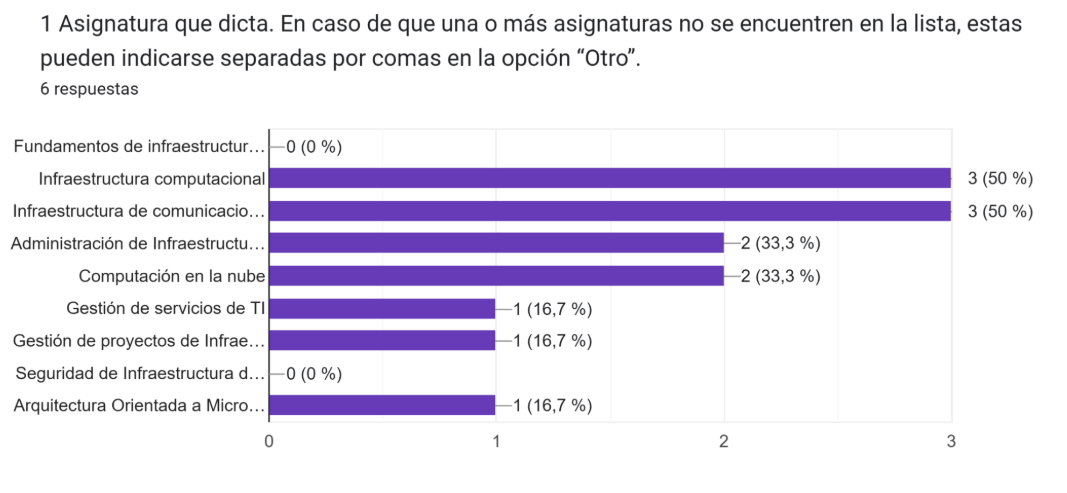
\includegraphics[scale=0.4] {tablas-images/cp1/pregunta1.png}
	\caption{Encuesta Docente | Asignatura que dicta}
	\label{fig:encuesta-docente-p1}
\end{figure}


\begin{itemize}
	\item El 50\% de los docentes imparte las asignaturas de Infraestructura Computacional e Infraestructura de Comunicaciones, estas asignaturas corresponden a aquellas donde se introducen por primera vez los conceptos de diseño relevantes para la notación a desarrollar.
	\item Existe una presencia significativa en áreas de vanguardia como Computación en la Nube y Administración de Infraestructura (33,3\% cada una), lo cual justifica la necesidad de que la (\NDITI) a desarrollar sea capaz de modelar entornos virtualizados y dinámicos.
	\item 
\end{itemize}

Esta alineación entre la investigación del GRID y el ejercicio docente facilita un escenario ideal para la validación práctica de la propuesta, permitiendo que las herramientas de modelado sean evaluadas por los estudiantes en contextos académicos

\subsection{Estado actual de las notaciones de diseño en el contexto académico}
Para profundizar en la caracterización de las necesidades del grupo, es necesario entender cómo se modelan actualmente sus soluciones de infraestructura al interior del programa de Ingeniería de Sistemas y Computación. Este análisis revela una fragmentación significativa que justifica la creación de una notación estandarizada.

\begin{figure}[H]
	\centering
	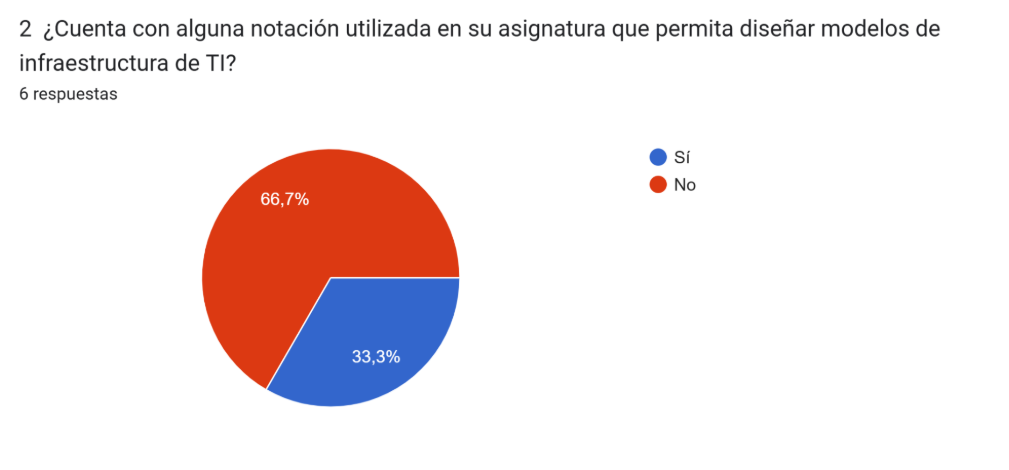
\includegraphics[scale=0.4] {tablas-images/cp1/pregunta2.png}
	\caption{Encuesta Docente | Notaciones usadas}
	\label{fig:encuesta-docente-p2}
\end{figure}

A pesar de la alta especialización de los integrantes del GRID, el análisis de las herramientas de modelado actuales revela una brecha importante en la estandarización de diseños de infraestructura, puesto que solo el 33,3\% de los docentes encuestados afirma contar con alguna notación utilizada en su asignatura que permita diseñar modelos de infraestructura de TI, mientras que la mayoría (66,7\%) no dispone de una herramienta específica para este fin.

\begin{figure}[H]
	\centering
	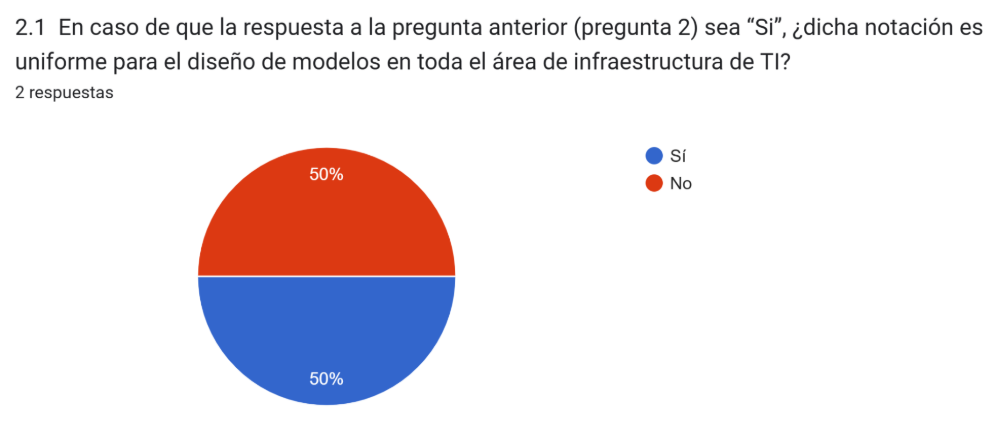
\includegraphics[scale=0.4] {tablas-images/cp1/pregunta2-1.png}
	\caption{Encuesta Docente | Notación uniforme}
	\label{fig:encuesta-docente-p2-5}
\end{figure}

\begin{figure}[H]
	\centering
	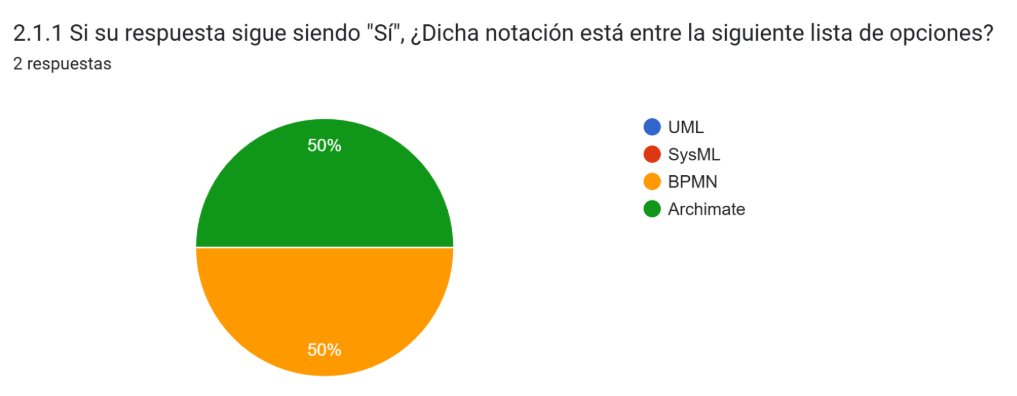
\includegraphics[scale=0.4] {tablas-images/cp1/pregunta2-2.png}
	\caption{Encuesta Docente | Nombre de la notación}
	\label{fig:encuesta-docente-p2-2}
\end{figure}

Adicionalmente, entre el grupo reducido que sí emplea notaciones, la percepción sobre la uniformidad es dividida: el 50\% considera que la notación es uniforme para todo el área de infraestructura, mientras que el otro 50\% sostiene que no lo es. Y a su vez, en los casos donde se aplica un estándar, el uso se reparte equitativamente (50\% cada uno) entre Archimate y BPMN.

La implementación de la notación permitiría unificar el 100\% de las asignaturas estratégicas bajo un mismo estándar, facilitando la comunicación entre los miembros de las asignaturas de manera que estos cuenten con una herramienta coherente que cubra los conceptos necesarios para el programa. 

\subsection{Preferencias y comodidad en el modelado de Infraestructura}
Al consultar a los investigadores sobre con qué notación se sentirían más cómodos para expresar los diagramas de sus asignaturas, los resultados son:

\begin{figure}[H]
	\centering
	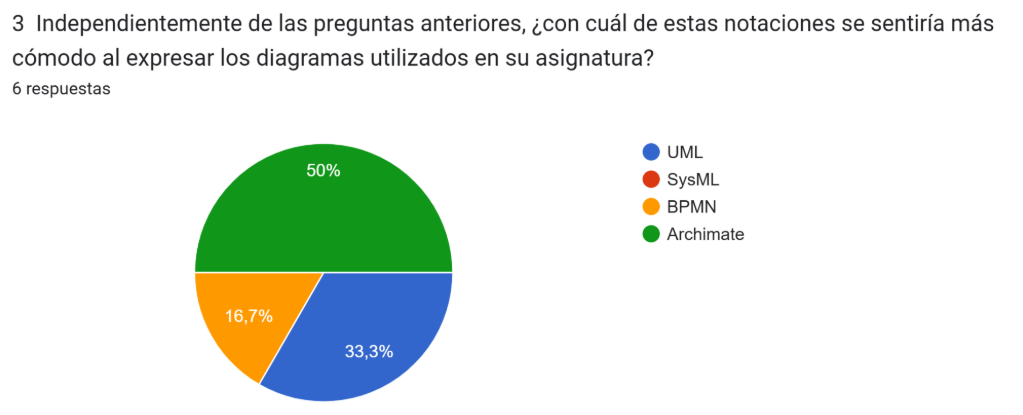
\includegraphics[scale=0.4] {tablas-images/cp1/pregunta3.png}
	\caption{Encuesta Docente | Comodidad con notaciones}
	\label{fig:encuesta-docente-p3}
\end{figure}

\begin{itemize}
	\item \textbf{Archimate:} Se posiciona como la opción preferida por el 50\% de los integrantes.
	\item \textbf{UML:} Ocupa el segundo lugar con un 33,3\% de preferencia.
	\item \textbf{BPMN:} Solo el 16,7\% se inclina por esta opción para representar infraestructura.
\end{itemize}

En cuanto a la percepción de comodidad en una escala de 1 a 5 (donde 5 es muy cómodo), la mayoría de los docentes muestra una actitud positiva hacia la adopción o mejora de herramientas de modelado:

\begin{figure}[H]
	\centering
	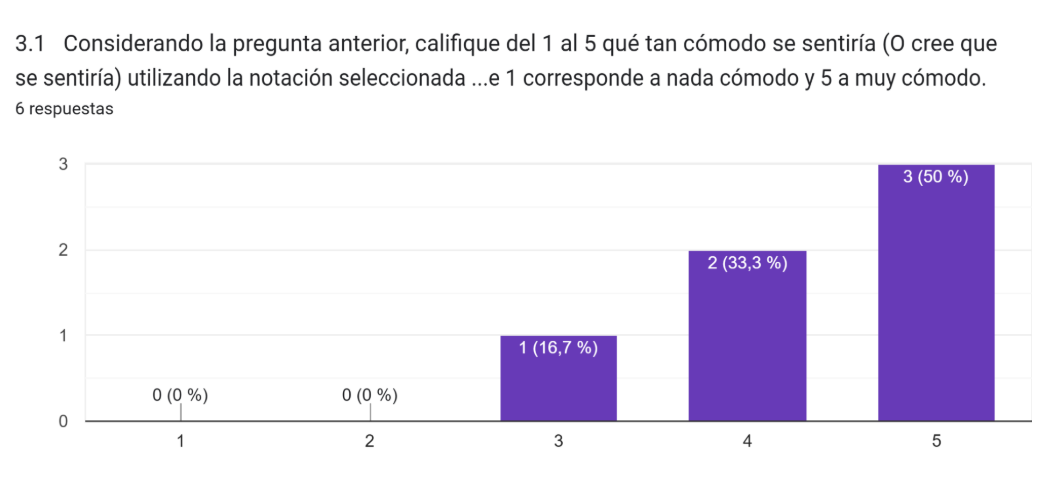
\includegraphics[scale=0.4] {tablas-images/cp1/pregunta3-1.png}
	\caption{Encuesta Docente | Calificación de notaciones}
	\label{fig:encuesta-docente-p3-1}
\end{figure}

\begin{itemize}
	\item El 50\% de los encuestados califica con un 5 su nivel de comodidad esperado al utilizar la notación de su preferencia.
	\item Un 33,3\% califica su comodidad con un 4, mientras que solo un 16,7\% mantiene una postura neutral (nivel 3).
\end{itemize}

Los anteriores datos sugieren que, si bien existe una base conceptual sólida en el \GRID, hay una carencia de herramientas compartidas. La preferencia mayoritaria por Archimate sugiere que la notación NDTi debería buscar una compatibilidad o lenguaje visual similar, pero enfocándose en resolver el vacío que deja el 66,7\% de docentes que actualmente no utiliza ninguna herramienta formal para el diseño de infraestructura.

\subsection{Requerimientos técnicos y funcionales de la notación}
Para garantizar que la propuesta NDTi sea pertinente, se consultó a los docentes sobre las dimensiones técnicas y las capas de abstracción que deben ser representadas en sus actividades académicas e investigativas.

El análisis de las capas trabajadas directamente en las asignaturas frente a aquellas que requieren una representación gráfica formal revela una necesidad de modelado integral. Según los resultados:

\begin{figure}[H]
	\centering
	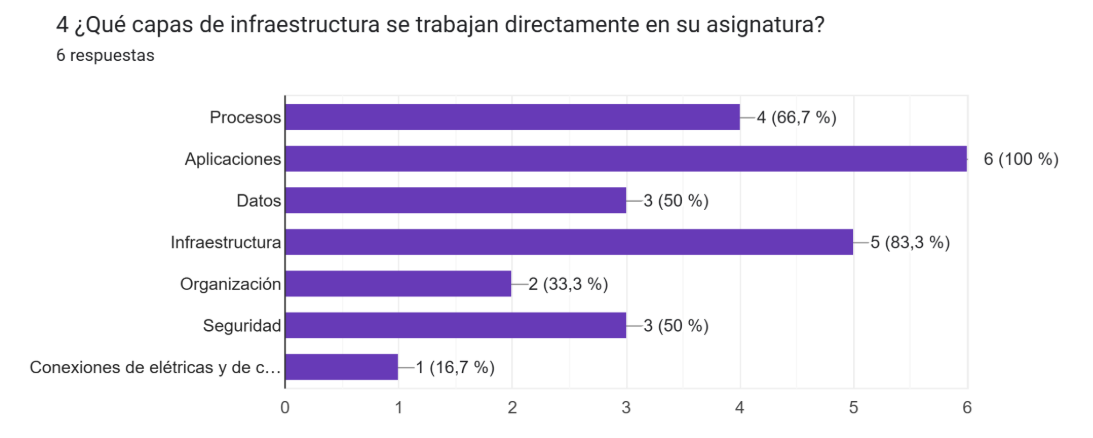
\includegraphics[scale=0.4] {tablas-images/cp1/pregunta4.png}
	\caption{Encuesta Docente | Capas de infraestructura}
	\label{fig:encuesta-docente-p4}
\end{figure}

\begin{figure}[H]
	\centering
	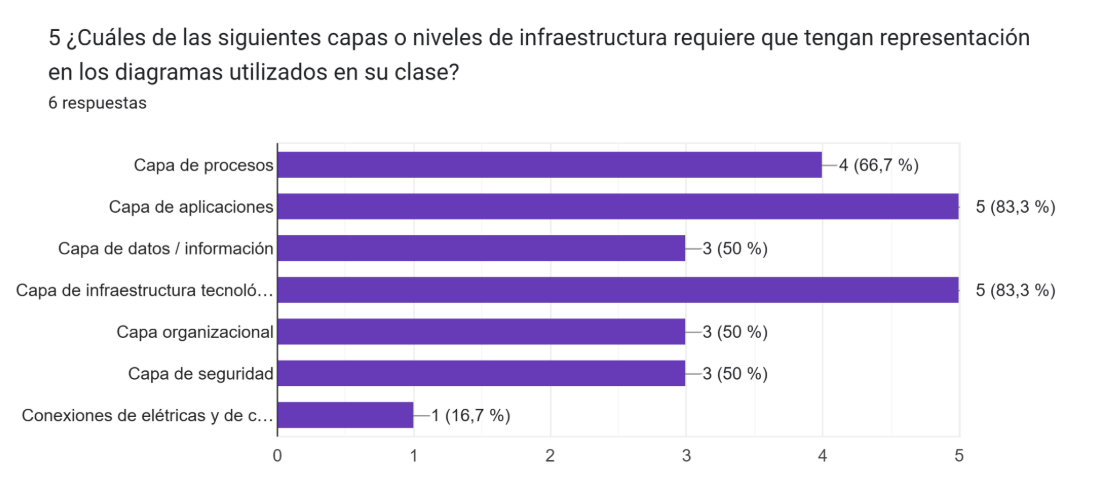
\includegraphics[scale=0.4] {tablas-images/cp1/pregunta5.png}
	\caption{Encuesta Docente | Representación de capas}
	\label{fig:encuesta-docente-p5}
\end{figure}

\begin{itemize}
	\item 100\% de los docentes trabaja directamente con la capa de Aplicaciones y un 83,3\% con la de Infraestructura. De manera coherente, un 83,3\% demanda que ambas capas tengan una representación explícita en los diagramas utilizados en clase.
	\item Existe una relevancia significativa en la capa de Procesos, trabajada por el 66,7\% de los docentes y requerida para modelado por la misma proporción (66,7\%). En cuanto a la capa de Datos/Información, el 50\% de los integrantes trabaja en ella y de igaul manera el 50\% exige su inclusión en el modelado técnico.
	\item Aunque el 50\% trabaja actualmente la capa de Seguridad y un 33,3\% la Organizacional, existe un consenso del 50\% de los docentes en que ambas dimensiones deberían estar representadas en los modelos.
\end{itemize}

Uno de los hallazgos más críticos para el diseño de la notación \NDITI es la forma en que los docentes perciben la conexión entre los diferentes componentes del sistema.

\begin{figure}[H]
	\centering
	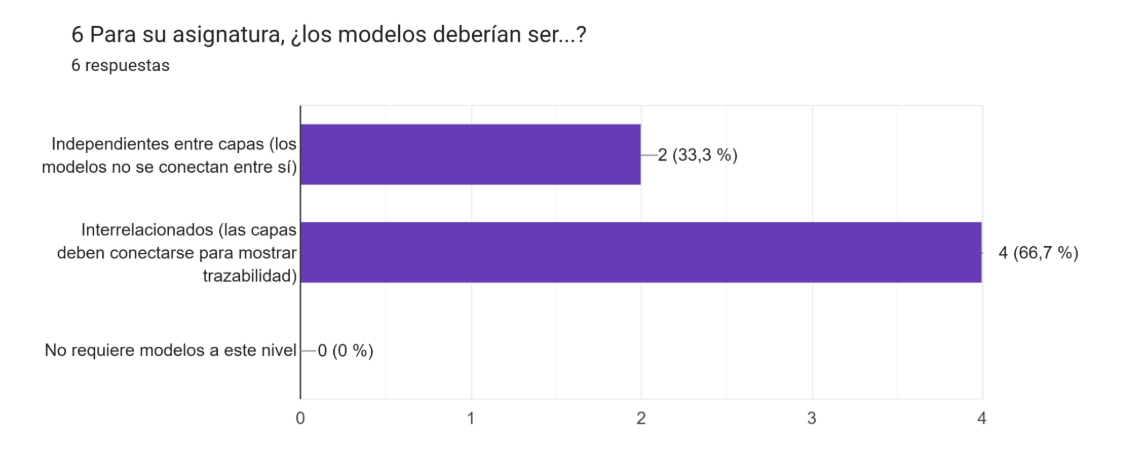
\includegraphics[scale=0.4] {tablas-images/cp1/pregunta6.png}
	\caption{Encuesta Docente | Necesidad de modelos}
	\label{fig:encuesta-docente-p6}
\end{figure}

\begin{itemize}
	\item El 66.7\% de los docentes sostiene que los modelos deben ser interrelacionados. Esto implica que las capas no deben verse como silos aislados, sino que la notación debe permitir mostrar la trazabilidad y la dependencia entre los mismos.
	\item El 33,3\% restante prefiere que los modelos mantengan independencia entre capas, eliminando en esta última medición la percepción de que no se requieren modelos a este nivel de detalle.
\end{itemize}

Los datos concluyen que la notación propuesta no debe limitarse únicamente a la representación de ``hardware'' o redes. Para satisfacer las necesidades del grupo docente, la \NDITI~debe ser una herramienta multicapa capaz de:

\begin{itemize}
	\item Articular la relación entre las diferentes capas o niveles de infraestructura de forma jerárquica o interrelacionada.
	\item Ofrecer una gramática visual que permita integrar conceptos de seguridad y procesos organizacionales a los modelos.
	\item Mantener una coherencia técnica que facilite la trazabilidad, permitiendo que los docentes o estudiantes de un área específica pueda entender y conectar los diseños de un área diferente.
\end{itemize}

\subsection{Análisis de experiencia previa y falencias en el modelado}

Para fundamentar la creación de una nueva propuesta, se evaluó experiencia de los docentes con las herramientas existentes, lo cual revela que, si bien hay un uso moderado de ciertos estándares, las dificultades técnicas y pedagógicas persisten.

El uso de lenguajes de modelado en las asignaturas de infraestructura ha estado dominado por herramientas tradicionales de ingeniería de software, sin embargo se ha cuestionado su suficiencia:

\begin{figure}[H]
	\centering
	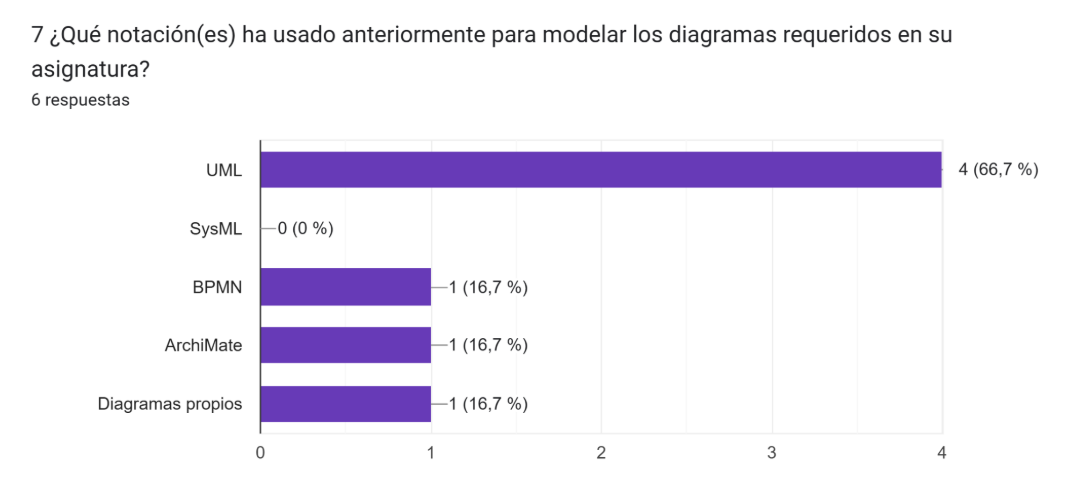
\includegraphics[scale=0.4] {tablas-images/cp1/pregunta7.png}
	\caption{Encuesta Docente | Notaciones usadas previamente}
	\label{fig:encuesta-docente-p7}
\end{figure}

\begin{figure}[H]
	\centering
	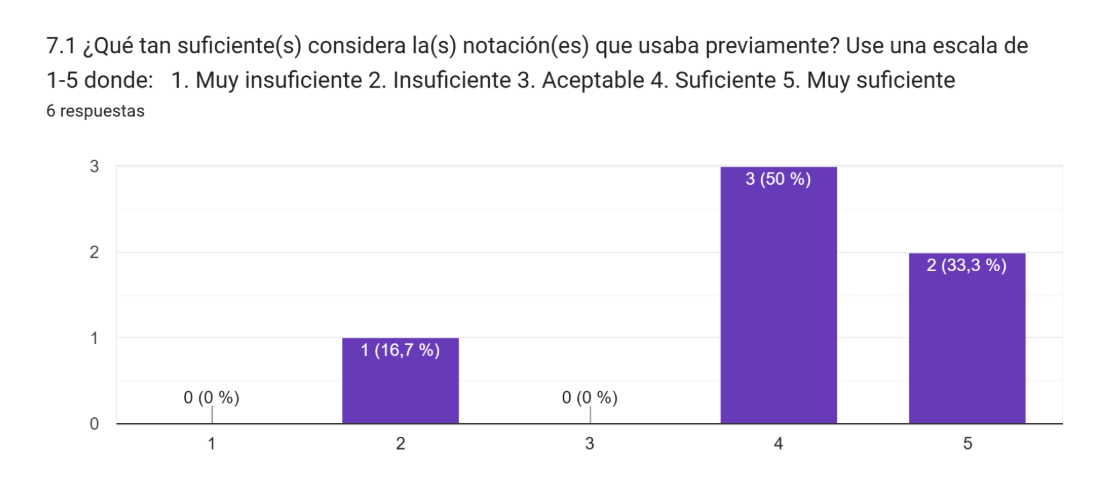
\includegraphics[scale=0.4] {tablas-images/cp1/pregunta8.png}
	\caption{Encuesta Docente | Suficiencia de las notaciones}
	\label{fig:encuesta-docente-p7-1}
\end{figure}

\begin{itemize}
	\item El 66,7\% de los docentes ha utilizado UML anteriormente para modelar diagramas de sus asignaturas, seguido por un uso minoritario de BPMN, ArchiMate y diagramas propios, con un 16,7\% cada una de estas opciones.
	\item La calificación promedio de estas notaciones es de 4.00 sobre 5. Aunque el 83,3\% las considera ``Suficientes'' (50\%) o ``Muy suficientes'' (33,3\%), un 16,7\% las califica como ``Insuficientes'', lo que indica que no cubren todas las necesidades del área de infraestructura.
\end{itemize}

El promedio mencionado anteriormente no elimina la necesidad de una notación específica. Como se analizó anteriormente, incluso quienes otorgan calificaciones altas identifican una falta de claridad en ciertos tipos de infraestructura y limitaciones para representar componentes técnicos, lo que ratifica que las notaciones generales no logran cubrir la totalidad de las necesidades del área.

Adicionalmente los docentes reportan obstáculos críticos que limitan la efectividad de las notaciones actuales en el aula de clase

\begin{figure}[H]
	\centering
	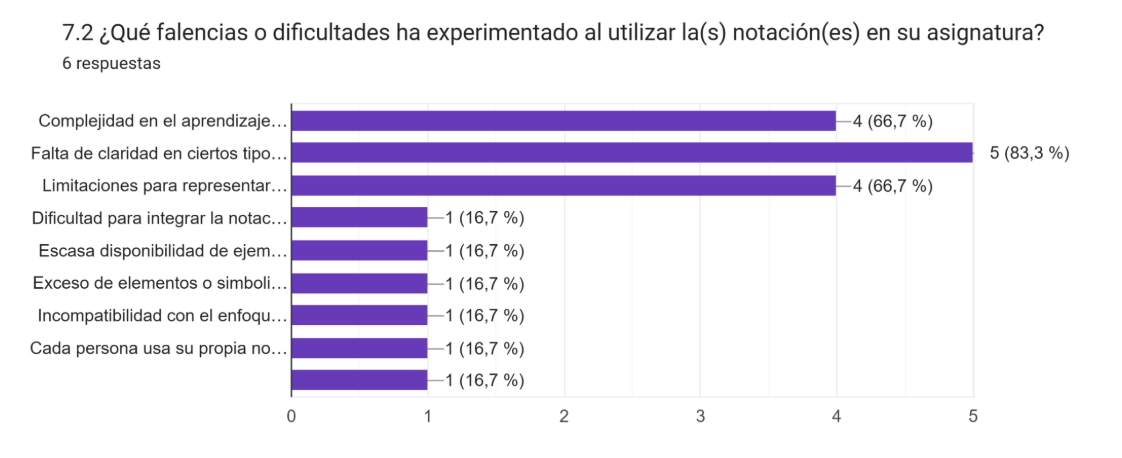
\includegraphics[scale=0.4] {tablas-images/cp1/pregunta9.png}
	\caption{Encuesta Docente | Problemáticas de las notaciones}
	\label{fig:encuesta-docente-p7-2}
\end{figure}

\begin{itemize}
	\item El 83,3\% de los encuestados coincide en que las herramientas actuales presentan una falta de claridad en ciertos tipos de infraestructura. Asimismo, un 66,7\% identifica limitaciones para representar componentes técnicos específicos.
	\item El 66,7\% identifica la complejidad en el aprendizaje de la simbología como una barrera significativa para los estudiantes.
	\item Se destaca que la existencia de diversos símbolos con el mismo significado genera confusión en el aula, dificultando que los estudiantes establezcan un estándar claro de representación.
\end{itemize}

La caracterización concluye con una serie de requerimientos funcionales que los expertos consideran esenciales para el éxito del proyecto:

\begin{figure}[H]
	\centering
	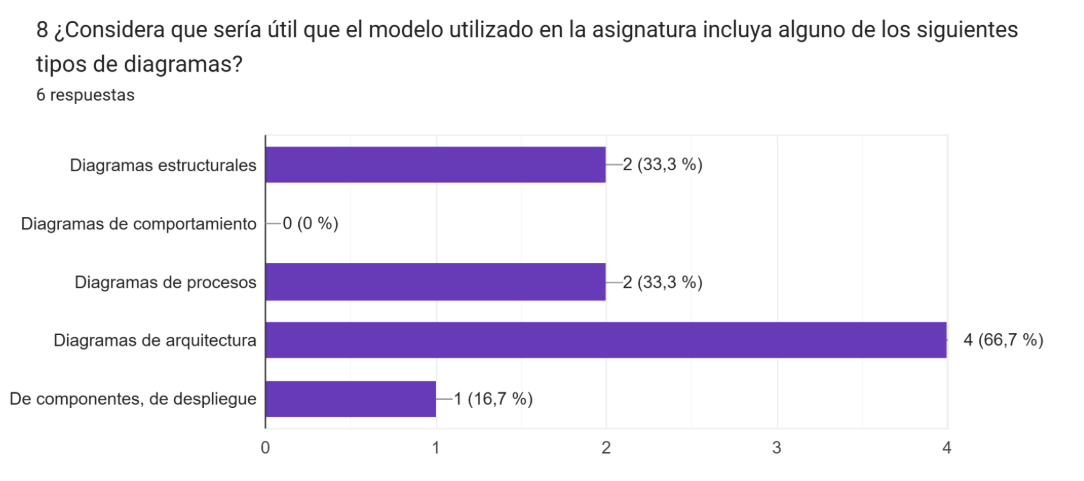
\includegraphics[scale=0.4] {tablas-images/cp1/pregunta10.png}
	\caption{Encuesta Docente | Tipos de diagrama}
	\label{fig:encuesta-docente-p8}
\end{figure}

\begin{figure}[H]
	\centering
	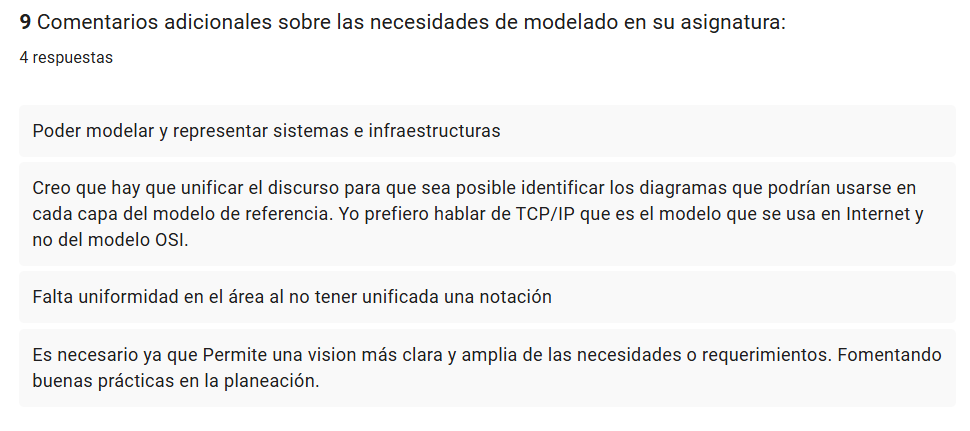
\includegraphics[scale=0.4] {tablas-images/cp1/pregunta11.png}
	\caption{Encuesta Docente | Comentarios adicionales}
	\label{fig:encuesta-docente-p9}
\end{figure}

\begin{figure}[H]
	\centering
	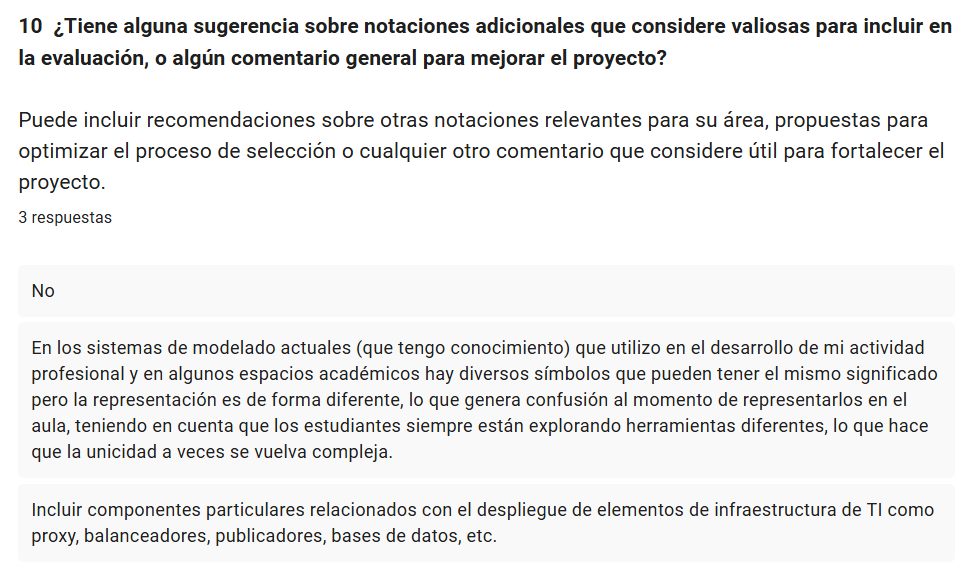
\includegraphics[scale=0.4] {tablas-images/cp1/pregunta12.png}
	\caption{Encuesta Docente | Sugerencias adicionales}
	\label{fig:encuesta-docente-p10}
\end{figure}

\begin{itemize}
	\item El 66,7\% de los docentes solicita priorizar los diagramas de arquitectura. Por su parte, un 33,3\% considera necesarios los diagramas estructurales y de procesos, mientras que solo un 16,7\% resalta la importancia de diagramas de componentes y de despliegue.
	\item Existe una necesidad explícita de incluir elementos particulares de despliegue relacionados a proxies, balanceadores o bases de datos. Estos componentes a menudo no se encuentran en notaciones de alto nivel como ArchiMate.
	\item Los comentarios finales subrayan la urgencia de unificar el discurso para identificar diagramas pertinentes en cada capa de los modelos de referencia. Se menciona una preferencia por el uso del modelo TCP/IP sobre el modelo OSI para alinearse con los estándares actuales de Internet.
	\item Los docentes enfatizan que una notación unificada permitirá una visión más clara y amplia de los requerimientos de infraestructura, eliminando la confusión generada por la existencia de diversos símbolos con el mismo significado. Lo que a su vez peude contribuir a reducir la complejidad en el aprendizaje para los estudiantes.
\end{itemize}

Con esta información, queda altamente justificada la necesidad de una nueva notación como una solución que equilibre la formalidad de un estándar de arquitectura con la especificidad técnica requerida por ciertos docentes, facilitando tanto la labor de los mismos, como la transferencia de conocimiento hacia los estudiantes.
%%%%% ##############################################################################################################################
%%%%% ##############################################################################################################################
%%%%% ##############################################################################################################################
%%%%% #############################################################################################################################
